\section{Location Estimators}\label{sec:estimators}
This section begins with a description of the distance metrics the result as a consequence of which geometry is chosen.  It then describes four estimators for the location parameter $\bm{S}\in SO(3)$ from orientation data generated by (\ref{eqn:1}) based on the two geometric choices (i.e., embedding (\ref{d_E})  in Sections~\ref{subsec:pam} and \ref{subsec:med} or intrinsic (\ref{d_R}) in Sections~\ref{section:ltwo} and \ref{subsec:lone}) and two decision-theoretic loss functions (i.e., squared distances in Sections~\ref{subsec:pam} and \ref{section:ltwo} or pure distances in Sections~\ref{subsec:med} and \ref{subsec:lone}).    The extent to which the choice of geometry or loss function matters in the estimation of $\bm{S}$ will be an important aspect explored in Section~\ref{ch:simulation}.  A summary of the four estimators and their properties is given in Table~\ref{tab:ests.sum}.


\subsection{Choice of Distance Metrics}\label{subsec:metrics}

The choice of geometry, i.e. Riemannian (non-Euclidean) or Euclidean, results in two different metrics to measure the distance
between two rotation matrices $\bm{R}_1$ and $\bm{R}_2 \in SO(3)$. Under the embedding approach, the natural distance
metric between two random matrices is the Euclidean distance, $\Edist $, which is induced by the Frobenius norm
\begin{equation}
\label{d_E}
\Edist (\bm{R}_1,\bm{R}_2)=\|\bm{R}_1-\bm{R}_2\|_F, 
\end{equation}
where $\|\bm{A}\|_F = \sqrt{\mathbf{tr}({\bm A^\top \bm A})}$ denotes the Frobenius norm of a matrix $\bm A$ and $\mathbf{tr}(\cdot)$ denotes the trace of a matrix.  The Euclidean distance between two rotation matrices corresponds to the shortest cord in $\M(3)$  that connects them.  If $r\in[0,\pi]$ denotes the misorientation angle in the angle-axis representation (\ref{eqn:angleaxis}) of $\bm{R}_1^\top \bm{R}_2 \equiv \bm{R}_1^\top \bm{R}_2(r,\bm{U})$ (so that $\mathbf{tr}(\bm{R}_1^\top \bm{R}_2) =1 +2 \cos r$), then $\Edist (\bm{R}_1,\bm{R}_2) = 2\sqrt{(1-\cos r)}$ holds.

By staying in the Riemannian space $SO(3)$ under the intrinsic approach, the natural distance metric becomes the Riemannian (or geodesic) distance, $\Rdist $, by which the distance between two rotations $\bm{R}_1,\bm{R}_2\in SO(3)$  is  defined as
\begin{equation}
\label{d_R}
\Rdist (\bm{R}_1,\bm{R}_2)=  \frac{1}{\sqrt{2}}||
\Log(\bm{R}_1^\top\bm{R}_2)||_F = r,
\end{equation}
where $\Log(\bm{R})$ denotes the principle logarithm of $\bm{R}$ (i.e., $\Log(\bm{R}) = \Log(\bm{R}(\bm U,r))= \bm \Phi(r\bm U)$ in \eqref{eqn:angleaxis}) and $r\in[0,\pi]$   is the misorientation angle of $\bm{R}_1^\top \bm{R}_2$.  The Riemannian distance corresponds to the length of the shortest path that connects $\bm{R}_1$ and $\bm{R}_2$ {\it within} the space $SO(3)$. For this reason, the Riemannian distance is often considered the more natural metric on $SO(3)$; see \cite{moakher02} for this discussion along with more details on exponential/logarithmic operators related to $SO(3)$.    
 
To make the difference between the Euclidean and Riemannian metrics more concrete, consider the lower dimension example given in Figure \ref{fig:dEvsdG}.  Here we plot two points, $\bm R_1,\bm R_2$, to visualize the endpoints of two rotations on $SO(2)$.  The Riemannian distance between them, $\Rdist (\bm R_1,\bm R_2)$,  is indicated by the thick black curved line.  As $\bm R_1\bm v$ rotates to $\bm R_2\bm v$ it does so along this curve therefore this distance is considered to stay in the space.  The Euclidean distance, $\Edist (\bm R_1,\bm R_2)$, is illustrated by the straight gray line.  It is impossible for $\bm R_1\bm v$ to move along this line, meaning we must leave $SO(2)$ in order to compute this distance.

\begin{figure}[h!]
\begin{center}
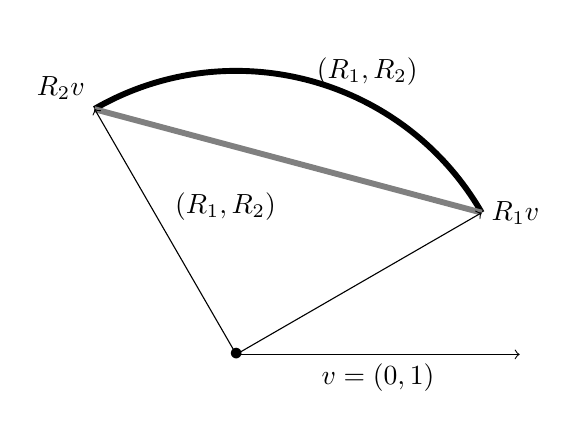
\begin{tikzpicture}[scale=.9]
%\draw (0,0) circle (4cm);
\draw (0,0) node {$\bullet$};
\draw (3.464102,2) node[anchor =  west]{$\bm R_1\bm v$};
\draw [->] (0,0)--(4,0);
%\draw [->] (4,0) arc (0:30:4cm);
\draw (2,0) node[anchor = north]{$\bm v=(0,1)$};
\draw (-2,3.46) node[anchor = south east]{$\bm R_2\bm v$};
\draw [line width=.75mm] (3.464102,2) arc (30:120:4cm);
\draw[line width=.75mm, color=gray] (-2,3.46)--(3.464102,2);
\draw [->](0,0) -- (-2,3.464102);
\draw [->](0,0)--(3.464102,2);
\draw (1,3.66) node[anchor= south west]{$\Rdist (\bm R_1,\bm R_2)$};
\draw (-1,1.75) node[anchor= south west]{$\Edist (\bm R_1,\bm R_2)$};
%\draw (0,0) circle (4cm);
%\draw (0,0) node {$\bullet$};
%\draw (0,0)--(4,0) node[anchor =  west]{$o_1$};
%\draw (4,0) node[anchor =  west]{$\bm R_1$};
%\draw (0,0)--(-2,3.46) node[anchor = south east]{$o_2$};
%\draw (-2,3.46) node[anchor = south east]{$\bm R_2$};
%\draw[line width=.75mm] (4,0) arc (0:120:4cm);
%\draw[line width=.75mm, color=gray] (-2,3.46)--(4,0);
%\draw (0,0)--(2,3.46) node[anchor= south west]{$\alpha$};
%\draw (2,3.46) node[anchor= south west]{$\Rdist (\bm R_1,\bm R_2)$};
%\draw (-1.25,0.73) node[anchor= south west]{$\Edist (\bm R_1,\bm R_2)$};
%\draw (3/8,.7)[->] arc (60:120:.75cm);
%\draw (0,1.2) node {$\frac{\alpha}{2}$};
%\draw (0,2.8) node {$\frac{\beta}{2}$};
%\draw (2,0) node[anchor=north]{1};
\end{tikzpicture}
\end{center}
\caption{An illustration of the difference between the Euclidean and Riemannian distance metrics on $SO(2)$.}
\label{fig:dEvsdG} 
\end{figure}


\subsection{The projected arithmetic mean}
\label{subsec:pam}

We begin with the definition of the arithmetic mean for orientation data, as its analog is most frequently encountered in the statistical literature for directional data \citep[e.g. see][]{mardia00}.   For a sample of $n$ random rotations $\bm{R}_i\in SO(3)$, $i=1,2,\dots,n$, this mean-type estimator is defined as
\begin{equation}\label{est:pam}
\ProjMean=\argmin_{\bm{S}\in
SO(3)}\sum_{i=1}^n\Edist^2(\bm{R}_i,\bm{S})=\argmax_{\bm{S}\in
SO(3)}\tr(\bm{S}^{\top}\bar{\bm{R}})
\end{equation}
where $\bar{\bm{R}}=\frac{1}{n}\sum_{i=1}^n\bm{R}_i$. The estimator is obtained by minimizing the sum of the squared distances in the Euclidean sense in the ambient space $\M(3)$, which then is projected back into $SO(3)$. \citet{moakher02}, who studied the mathematical characteristics of this estimator in detail, therefore refers to it as the \textit{projected arithmetic mean}.    This estimator's appeal lies in its simplicity and statistically intuitive nature, though it has been noted that the estimator is not invariant under rigid transformations \citep[see][]{moakher02}.  However, this estimator does correspond to the maximum likelihood estimator of $\bm{S}$ when the symmetrically distributed rotation errors in (\ref{eqn:1}) follow a matrix Fisher distribution \citep{jupp79}.  \citet{leon06} also derived this estimator as the method of moment estimator under a Cayley  distribution, and \citet{bingham09} showed that the projected arithmetic mean corresponds to the maximum quasi-likelihood estimator for orientation data with rotation errors arising from the circular-von Mises-based distribution.  

 \citet{arun87} and \citet{horn88} independently offered algorithms to find this matrix.  \citet{umeyama91} refined their solutions and also considered special cases such as $\det(\bar{\bm R})=0$.

\subsection{The projected median}
\label{subsec:med}

A modification of the estimator from Section~\ref{subsec:pam} is obtained by replacing the squared distances in \eqref{est:pam} with pure distances, leading to a median-type estimator defined as
\begin{equation}\label{est:med}
\ProjMedian=\argmin_{\bm{S}\in
SO(3)}\sum_{i=1}^n\Edist(\bm{R}_i,\bm{S}).
\end{equation}
For rotation data, we refer to this estimator of $\bm{S}$ as the \textit{projected median}.  
The analog of this estimator for spherical data has been considered by \citet{chan93} (i.e., the so-called normalized spatial median of \cite{ducharme87}) for estimating the central direction of data points on the sphere.   Those authors found the estimator to be preferable for spherical data following the Fisher model on the sphere. For additional information on (\ref{est:med}) and related estimators for directional data (e.g. the mediancentre \citep{gower74} or the Weber point \citep{bajaj88}),  see \citet{durocher09}. 

An algorithm to compute this estimator hasn't been proposed as of this writing, so we detail our method here.  Our method is based on the Weiszfeld algorithm originally given by \cite{weiszfeld37}.  The algorithm requires an initial value that does not equal any sample point. For the purpose of speeding up computing time we use $\ProjMean$ as the starting point. Note that the solution is generally not sensitive to the choice of starting points unless the data exhibit extreme spread.
\begin{enumerate}
\item Set $\widehat{\bm S}=\ProjMean$ and choose an arbitrarily small stopping rule $\varepsilon$.
\item For $i=1,\ldots,n$ compute $\bm s_i=\bm R_i-\widehat{\bm S}$.
\item Calculate
\[
\bar{\bm R}_W=\frac{\sum_{i=1}^n\bm R_i/||\bm s_i||_F}{\sum_{i=1}^n1/||\bm s_i||_F}
\]
which we call the weighted mean with respect to $\widehat{\bm S}$.
\item Define $\widehat{\bm S}_{\text{new}}$ to be the $\mathcal{M}(3)$ projection of $\bar{\bm R}_W$.
\item If $\varepsilon>||\widehat{\bm S}-\widehat{\bm S}_{\text{new}}||_F$ return $\ProjMedian=\widehat{\bm S}_{\text{new}}$; otherwise set $\widehat{\bm S}=\widehat{\bm S}_{\text{new}}$ and return to step 2.
\end{enumerate}

\subsection{The geometric mean}
\label{section:ltwo}
As sketched in Section~\ref{subsec:geometry}, the Lie group property of $SO(3)$ provides us with a convenient transform from $SO(3)$
into the tangent space $\mathfrak{so}(3)$ that is closed under
addition and scalar multiplication.  Obtaining the median or mean
in this transformed space and projecting the result back to $SO(3)$ corresponds to the rotation that minimizes the first and second order Riemannian
distances, respectively \citep{karcher77, moakher02, fletcher08, fletcher09}.  \citet{karcher77} made use of Riemannian manifolds to compute what is often called the Riemannian
center of mass.  \citet{moakher02} applied Karcher's ideas to
rotation matrices and defined
\begin{equation}\label{est:ltwo}
\GeomMean=\argmin_{\bm{S}\in
SO(3)}\sum_{i=1}^n\Rdist^2(\bm{R}_i,\bm{S}).
\end{equation}
which was termed as the \textit{geometric mean}.  Note that the solution to  \eqref{est:ltwo} may not be
unique. Uniqueness is tied to the property of geodesic convexity of the objective function in \eqref{est:ltwo}. For more information, we refer to \citet{moakher02}.  Additionally, \eqref{est:ltwo} generally does not have a closed-form solution making this estimator much more computationally intensive than its Euclidean counterpart (the projected arithmetic mean of Section~\ref{subsec:pam}).  The algorithm proposed by \citet{manton04} was used in our simulation study.

\subsection{The geometric median}
\label{subsec:lone}
The median-type counterpart to the geometric mean was defined first in the context of
spherical data by \citet{fisher85} as the point on the sphere that minimizes the sum of the arc lengths to all
observations in the sample.   For this type of data, the resulting estimator is known as the spherical median,
 which is a special case of the generalized median in $\R^d$
proposed by \citet{gower74}.   For spherical data, an alternative formulation to the
spherical median has been given by \citet{liu92} in the framework of
data depth leading, however, to the same solution.

We give an adaptation of the spherical median to rotation matrices. 
Recall that the shortest geodesic path between two rotations ${\bm R_1}$, ${\bm R_2}$ is given by the Riemannian distance $\Rdist(\bm R_1,\bm R_2)$.  Thus the rotation matrix analog of the \cite{fisher85} spherical
median can be defined as
\begin{equation}\label{est:lone}
\GeomMedian=\argmin_{\bm{S}\in
SO(3)}\sum_{i=1}^n\Rdist(\bm{R}_i,\bm{S});
\end{equation}
see also \cite{fletcher08, fletcher09}.  We refer to this estimator of $\bm{S}$ as the \textit{geometric median.}  \citet{hartley11} offers an algorithm to find the geometric median in $SO(3)$.


\begin{table}[h]
\caption{A summary of the estimators presented and their properties.  \label{tab:ests.sum}}
\begin{center}
\begin{tabular}{ lclclcl}\hline
\rule[2mm]{0mm}{1mm} \textbf{name} & & \textbf{symbol} & & \textbf{distance metric} &&\textbf{cost function}\\ \hline \hline 
\rule[2mm]{0mm}{6mm} Projected Arithmetic Mean & & $\ProjMean$ & & Euclidean &&$\sum_{i=1}^n\Edist^2$  \\
\rule[2mm]{0mm}{6mm} Projected Median & & $\ProjMedian$ & & Euclidean && $\sum_{i=1}^n\Edist$ \\
\rule[2mm]{0mm}{6mm} Geometric Mean & & $\GeomMean$&  & Riemannian && $\sum_{i=1}^n\Rdist^2$\\0
\rule[2mm]{0mm}{6mm} Geometric Median & & $\GeomMedian$&  & Riemannian &&$\sum_{i=1}^n\Rdist$ \\[-7mm] 
\rule[2mm]{0mm}{6mm} & & & & \\ \hline
\end{tabular}
\end{center}
\end{table}
